\documentclass[10pt]{article}

\usepackage[utf8]{inputenc}
\usepackage{floatrow}

\usepackage{algorithm, algpseudocode}
\let\oldReturn\Return
\renewcommand{\Return}{\State\oldReturn}
\newcommand{\N}{\mathbb{N}}
\newcommand{\R}{\mathbb{R}}
\usepackage[T1]{fontenc}
\usepackage{enumitem}
\usepackage{hyperref}
\usepackage{scrextend}
\usepackage{amsmath}
\usepackage{amsfonts}
\usepackage{stmaryrd}
\usepackage{graphicx}
\usepackage{eurosym}
\usepackage{color}
\usepackage{listings}
\usepackage{wrapfig}
\usepackage{array}
\usepackage[hmargin=1.25in,vmargin=1.25in]{geometry}

% table of contents setup
\renewcommand{\contentsname}{Sommaire}
\usepackage{etoolbox}
\patchcmd{\thebibliography}{\section*{\refname}}{}{}{}

\usepackage[utf8]{inputenc}
\usepackage[T1]{fontenc}
\usepackage[frenchb]{babel}

\usepackage[T1]{fontenc}
\usepackage{beramono}% monospaced font with bold variant
 
\usepackage{listings}
\lstdefinelanguage{VHDL}{
   morekeywords={
     library,use,all,entity,is,port,in,out,end,architecture,of,
     begin,and
   },
   morecomment=[l]--
}
 
\usepackage{xcolor}
\colorlet{keyword}{blue!100!black!80}
\colorlet{comment}{green!90!black!90}
\lstdefinestyle{vhdl}{
   language     = VHDL,
   basicstyle   = \ttfamily,
   keywordstyle = \color{keyword}\bfseries,
   commentstyle = \color{comment}
}
 
 
\setlength{\parindent}{0cm}
\setlength{\parskip}{1ex plus 0.5ex minus 0.2ex}
\newcommand{\hsp}{\hspace{20pt}}
\newcommand{\HRule}{\rule{\linewidth}{0.5mm}}

\hypersetup{
    colorlinks,
    citecolor=black,
    filecolor=black,
    linkcolor=blue,
    urlcolor=red
}

\lstset{language=C,
                basicstyle=\ttfamily,
                keywordstyle=\color{blue}\ttfamily,
                stringstyle=\color{red}\ttfamily,
                commentstyle=\color{cyan}\ttfamily,
                morecomment=[l][\color{magenta}]{\#}
}

\begin{document}
    
    \begin{titlepage}
        \begin{sffamily}
            \begin{center}

                \begin{figure}[h!]
                    
\includegraphics[width=6cm]{ensiie.jpeg}
                \end{figure}

                \HRule \\[0.8cm]
                { \huge \bfseries Micro-architecture (UE S3) } \\[0.4cm]
                \HRule \\[2.0cm]
                
                { \huge \bfseries Dossier de Projet } \\[0.5cm]

                \textsc{\Large Serpentin 7-segment programmable (FPGA)}\\[2.0cm]

                \vfill
                \begin{minipage}{0.4\textwidth}
                    \begin{flushleft} \large
                        \emph{Etudiants:} \\
                        Afizullah \textsc{Rahmany}\\
                        Romain \textsc{Pereira}\\
                    \end{flushleft}
                \end{minipage}
                \begin{minipage}{0.4\textwidth}
                    \begin{flushright} \large
                        \emph{Enseignant:}  \\
                        M. \textsc{Augé}
                    \end{flushright}
                \end{minipage}
                \\[2.0cm]
                {\large 25/11/2018}
            \end{center}
        \end{sffamily}
    \end{titlepage}
    
    \tableofcontents
    \section*{Préambule}
    Ce projet a été réalisé dans le cadre de nos études à l'ENSIIE (Ecole National Supérieur d'informatique pour l'industrie et l'entreprise) d'Evry.
    
    Ce projet est l'aboutissement de nos cours en Micro-architecture.
    
    Nous programmions sur un FPGA d'Altera (gamme Cyclone), en VHDL et à l'aide du logiciel Quartus.
    
    L'objectif a été de réaliser un serpentin programmable, et affichable sur un 7-segment.

    \newpage
    \section{Introduction}
    Vous cherchez un cadeau de noël pour vos enfants ou vos grands parents?
    \newline
    Ne cherchez plus, voici \textbf{le Serpentin 3000}
    \newline
    Cette modeste plaquette électronique passionera les petits comme les grands enfants.
    \newline
    \newline
    \textbf{Amusez vous!}
    \newline
    Modifier la vitesse et le type de défilement.
    \newline
    \newline
    \textbf{Exprimez votre créativité!}
    \newline
    Grâce à l'interface 'Programmation 3000', vous pouvez créer votre propre serpentin.
    \newline
    \newline
    \textbf{Accessible}
    Pour la modique somme de 4.99\euro, offrez vous un\\
    \\
    \\
    \\
    \centerline{\textbf{SERPENTIN 3000}}
    \newline
    \newline
    \begin{figure}[h!]
        
\includegraphics[width=6cm]{logo.png}
    \end{figure}

    \newpage
    \section{Manuel utilisateur}
    
    \paragraph{Bouton de droite} 'Bouton reset' , réinitialise l'état du serpentin dans son état initial
    
    \paragraph{Interrupteurs} 'IVDF2 IVDF1 IVDF0' permettent de régler la vitesse de défilement (en nombre de ticks)
    
    \begin{table}[h]
        \centering
        \begin{tabular}{cccc}
                IVDF2 & IVDF1 & IVDF0 & vitesse de défilement \\
                  0   &   0   &   0   & 2 \\
                  0   &   0   &   1   & 5 \\
                  0   &   1   &   0   & 7 \\
                  0   &   1   &   1   & 10 \\
                  1   &   0   &   0   & 12 \\
                  1   &   0   &   1   & 15 \\
                  1   &   1   &   0   & 17 \\
                  1   &   1   &   1   & 20 \\
        \end{tabular}
    \end{table}
        
    \paragraph{Diodes d'interrupteurs} 'DVDF2 DVDF1 DVDF0' allumées ou éteintes selon que les interrupteurs IVDF2, IVDF1 ou IVDF0 sont actifs ou inactifs.
    
    \paragraph{Diode défilement} 'DVDF' cette diode clignote à la vitesse de défilement
    
    \paragraph{Sélectionneur serpentin} 'SEL1 SEL2' permettent de sélectionner le type de serpentin
    
    \begin{table}[h]
        \centering
        \begin{tabular}{cccc}
                SEL1 & SEL0 & type de serpentin \\
                  0  &   0  &    clignotement   \\
                  0  &   1  &    horaire        \\
                  1  &   0  &    anti-horaire   \\
                  1  &   1  &    programmable   \\
        \end{tabular}
    \end{table}
        
        
    \paragraph{BUS - IA} BUS-IA, prend un message pour communiquer avec le serpentin \ref{formatmsg}

    \newpage
    \section{Présentation générale}
    
        \subsection{Fonctionnement}
        \begin{figure}[h!]
            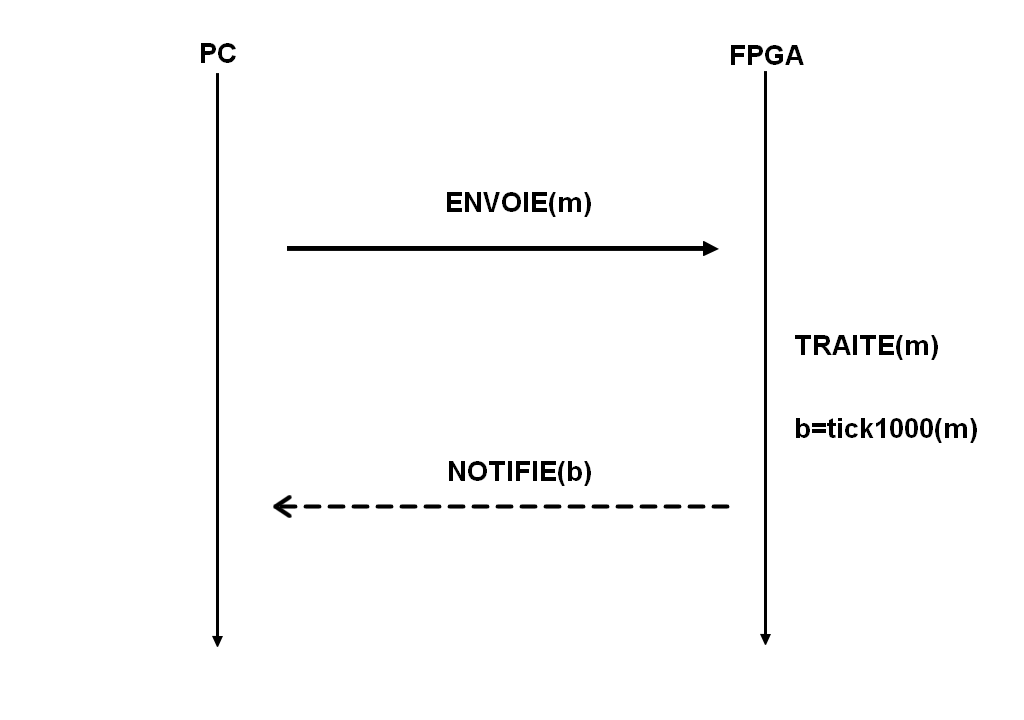
\includegraphics[width=7cm]{fonctionnement.png}
            \caption{MSC des actions utilisateur}
        \end{figure}
        
        \textbf{m} est un \textit{message}. Il s'agit d'une suite de \textbf{44 bits} avec le format:
        
        - \textbf{bits 43 à 24} Ce sont les bits du contrôle du BUS-IA (voir Bus-IA)
        
        - \textbf{bits 23 à 0} Ce sont les bits du message

        \begin{figure}[h!]
            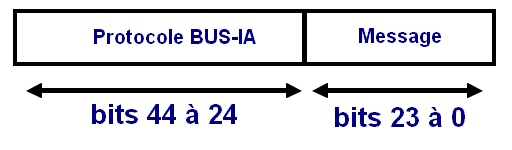
\includegraphics[width=10cm]{messages1.png}
        \end{figure}

        Un \textit{message} doit avoir le format:
        
        - \textbf{bits 23 à 21} Ce sont les bits codant le \textit{type} du \textit{message}
        
        - \textbf{bits 20 à 0} Ce sont les données du message, le format varie selon le \textit{type}
        
        \begin{figure}[h!]
            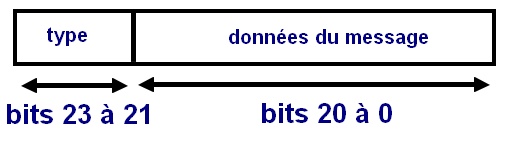
\includegraphics[width=10cm]{messages2.png}
        \end{figure}
        
        \newpage
        \subsection{Format des messages}\label{formatmsg}
        
        Ci-dessous, voici les commandes supportées par le processeur,
        et le format des messages permettant d'executer ces commandes.
        \newline
        \newline
        \textbf{noop} Ne rien faire
        
        - \textbf{bits 23 à 21} : ``000'' (= (bit 23, bit 22, bit 21))

        - \textbf{bits 20 à 0} : \textit{non utilisées}
        \newline
        \newline
        \textbf{h-init(n)} Génère un tick sur H100 tous les n coups d'horloge maître
        
        - \textbf{bits 23 à 21} : ``001''

        - \textbf{bits 20 à 0} : \textit{non utilisées}
        \newline
        \newline
        \textbf{h-check-ON()} Demande au processeur d'envoyer au PC un message TICK1000 tous les 1000 tickets de H100.
        
        - \textbf{bits 23 à 21} : ``010''

        - \textbf{bits 20 à 0} : \textit{non utilisées}

        \textbf{h-check-OFF()} Demande au processeur d'arrêter d'envoyer au PC un message TICK1000
        
        - \textbf{bits 23 à 21} : ``011''

        - \textbf{bits 20 à 0} : \textit{non utilisées}
        \newline
        \newline
        \textbf{clr()} Indique au processeur d'afficher un serpentin vide sur le 7-segment (\textbf{n} à 32 et met à 0 toutes les \textit{valeurs} programmées
        
        - \textbf{bits 23 à 21} : ``100''

        - \textbf{bits 20 à 0} : \textit{non utilisées}
        \newline
        \newline
        \textbf{set-N(n)} Indique au processeur le nombre de \textbf{valeurs} à faire défiler en boucle sur le 7-segments. (\textbf{n} compris entre 1 et 32)\label{N}
        
        - \textbf{bits 23 à 21} : ``101''

        - \textbf{bits 20 à 6} : \textit{non utilisées} 

        - \textbf{bits 5 à 0} : \textbf{n} codé sur 6 bits ($2^6 = 64$)
        \newline
        \newline
        \textbf{set-val(i, v)} Indique au processeur la i-ème valeur du 7-segments est \textbf{v}
        
        - \textbf{bits 23 à 21} : ``110''

        - \textbf{bits 20 à 13} : \textit{non utilisées} 

        - \textbf{bits 12 à 6} : \textbf{v} les 7 bits correspond aux 7 segments de l'afficheur (0 => éteint, 1 => allumé)

        - \textbf{bits 5 à 0} : \textbf{n} codé sur 6 bits ($2^6 = 64$)

    \newpage
    \section{Description matérielle}
    
        \subsection{Schéma général}

         Quelques simplifications ont eu lieu pour la lisibilité du schéma:
        
        - En réalité, chaque bloc prend la master clock et le bouton reset en entrée
        
        - Les 224 bits de configuration et les 6 bits codant N ont été groupé en un seul fil (de 230 bits)
        
        - S6 S5 S4 S3 S2 S1 S0 sont combinés en un seul fil

        \begin{figure}[h!]
            \hspace*{-2cm}                                                          
            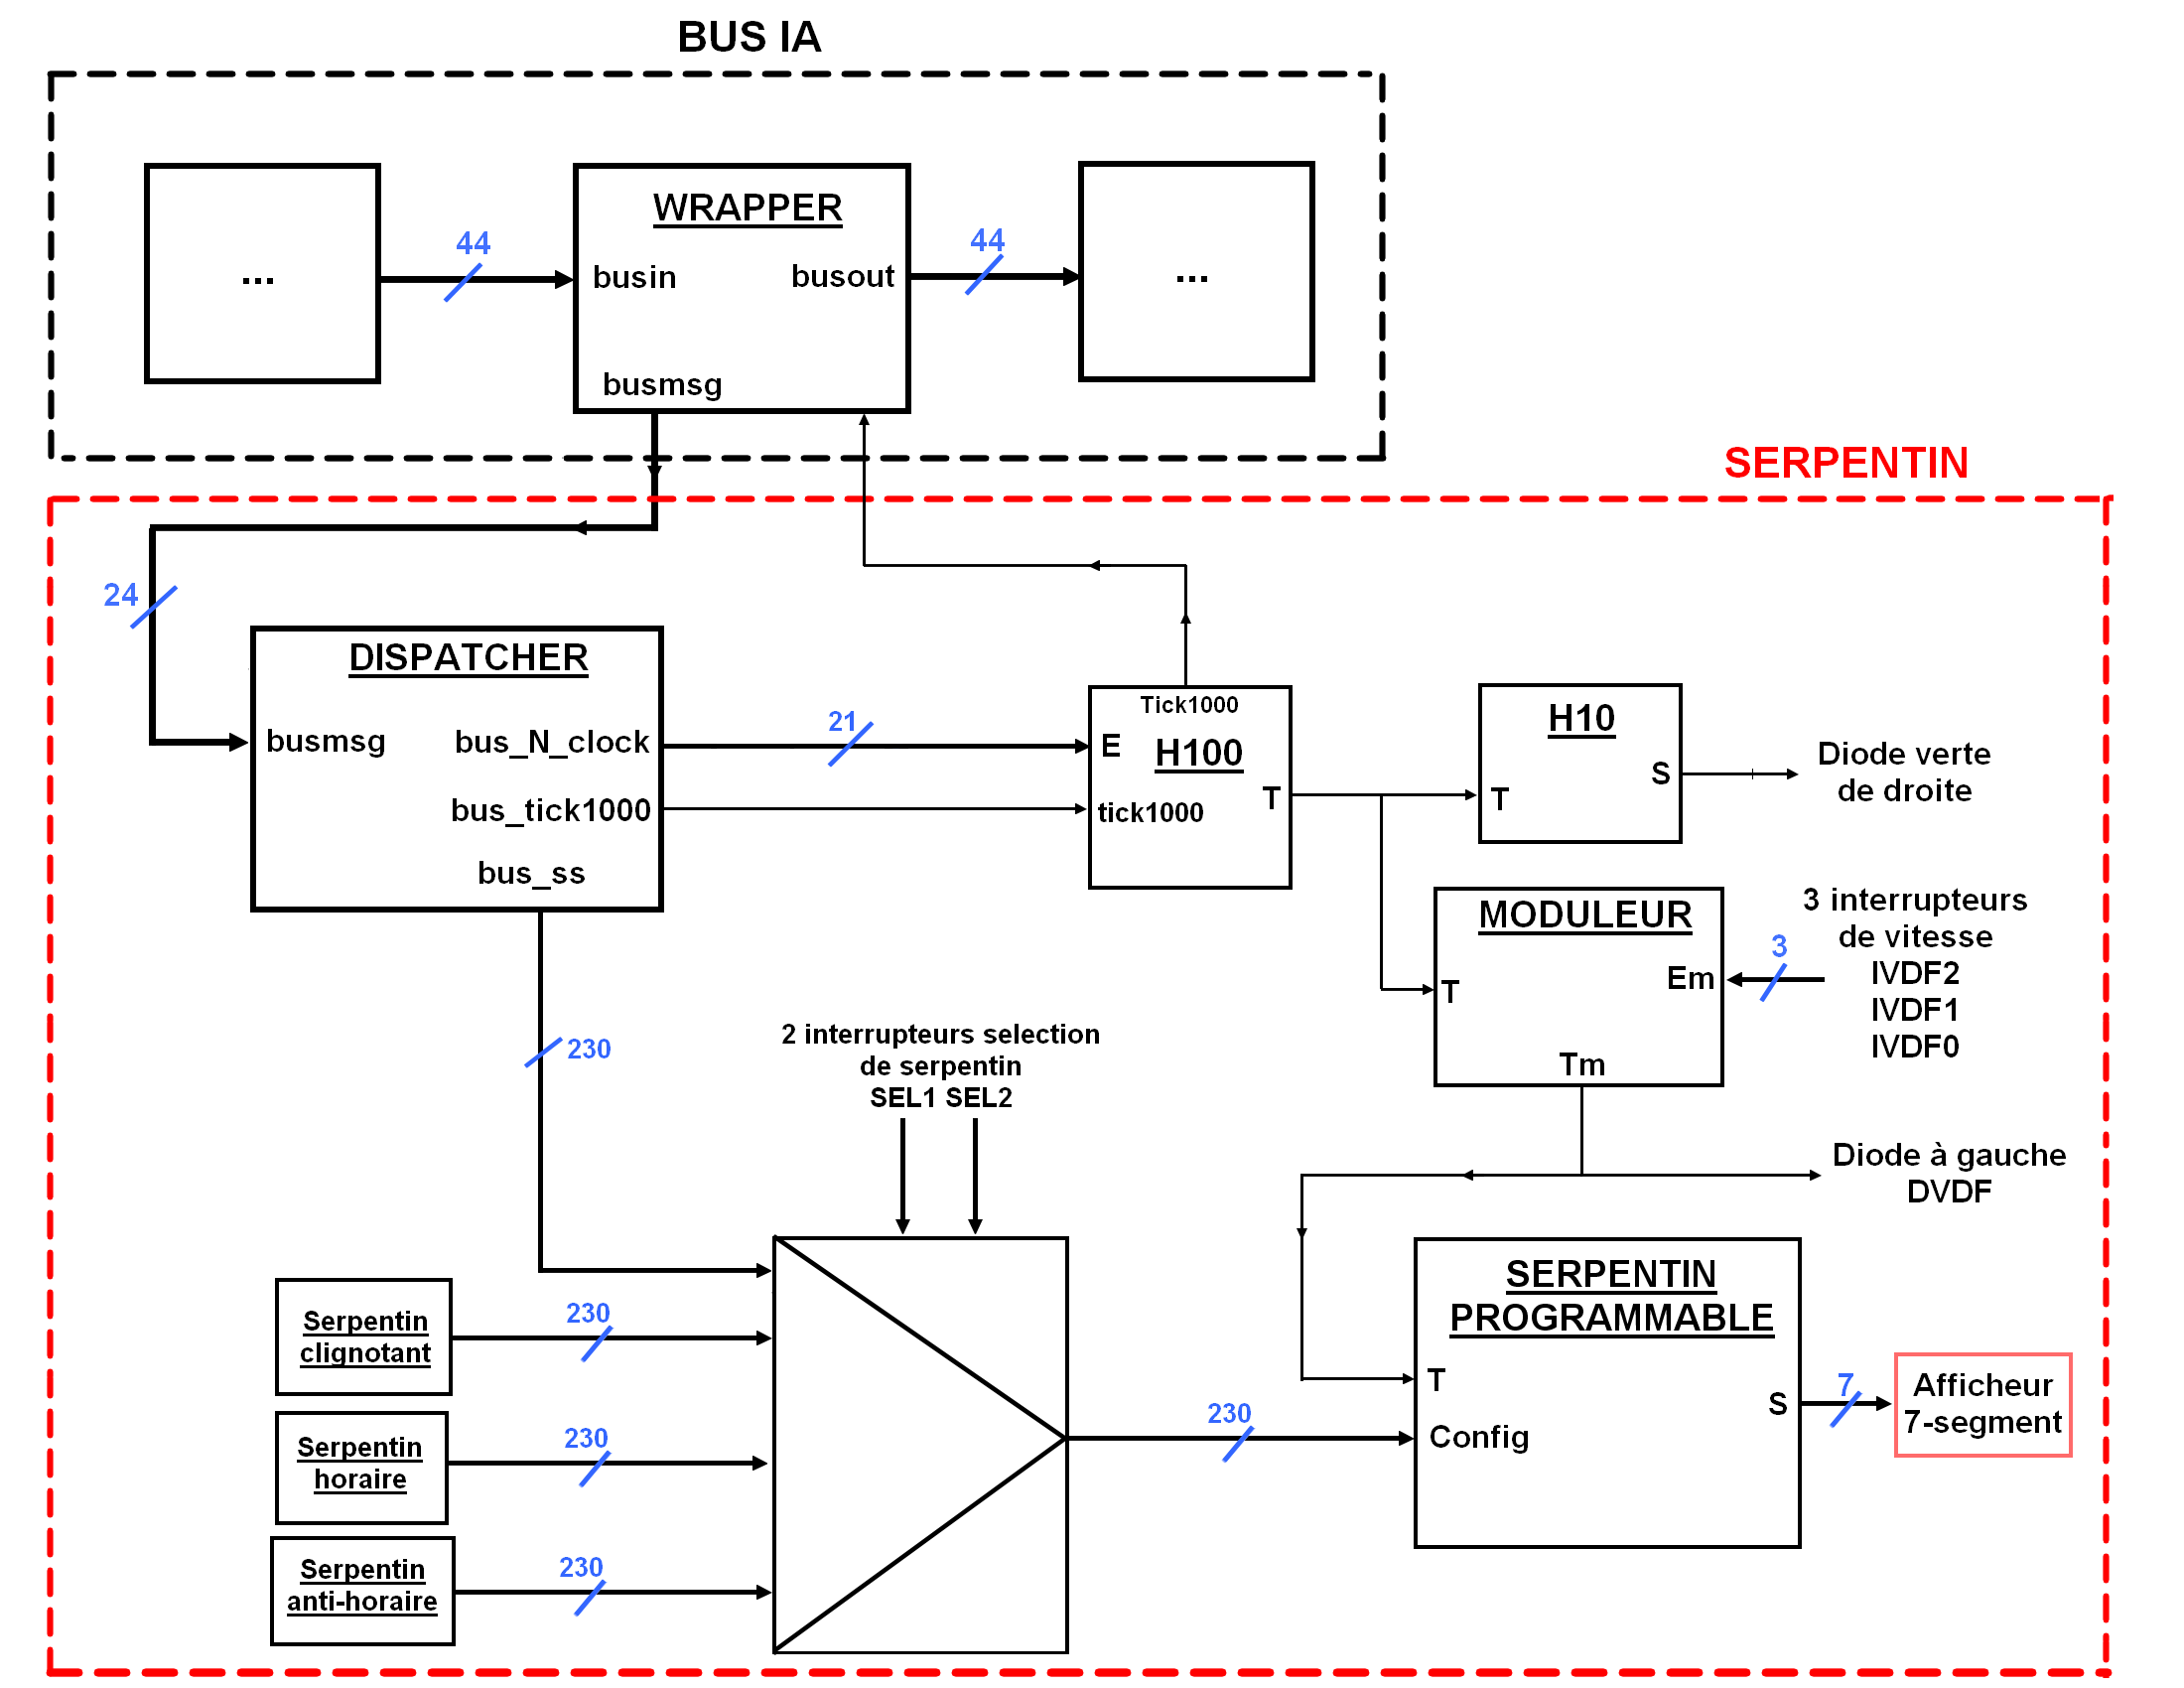
\includegraphics[width=20cm]{schema.png}
            \caption{Schéma général simplifié du matériel}
        \end{figure}

    \newpage
    \subsection{Description des blocs}
        
        \subsubsection{Wrapper}
        
        Il s'agit de l'interface de communication dans le BUS-IA.
        
        Ce bloc suit le protocole 'handshake' dans le BUS-IA.
        
        Il récupère les messages qui lui sont destinés,
        puis les renvoie vers le processeur du serpentin.
        
        \textbf{Entrées}
        
            - clk, reset : la master clock et le reset
            
            - busin : entrée dans le BUS-IA (44 bits, protocole handshake)
            
            - busin\_valid : entrée dans le BUS-IA (1 bit, protocole handshake)

            - busout\_eated : entrée dans le BUS-IA (1 bit, protocole handshake)
                            
        \textbf{Sorties}
            
            - busout : sortie vers le BUS-IA (44 bits, protocole handshake)
           
            - busout\_valid : sortie vers le BUS-IA (1 bit, protocole handshake)
           
            - busin\_eated : sortie vers lle BUS-IA (1 bit, protocole handshake)

            - busmsg : sortie vers le processeur du serpentin (24 bits, pas de protocole)


        
        \subsubsection{Dispatcher}
        
        Il s'agit du bloc de répartition.
                
        Il récupère les \textit{messages} qui lui sont destinés,
        les interprète, et modifie ses sorties en fonction.
        
        \textbf{Entrées}
        
            - clk, reset : la master clock et le reset
            
            - busmsg : le message a interpreté (24 bits)
                            
        \textbf{Sorties}
            
            - bus\_ss : sortie vers le 7-segment (32 * 7 + 6 = 224 bits), codant les configurations possibles du 7-segments.
           
            - bus\_n : sortie vers le 7-segment (6 bit), codant 'N' (\ref{N})

            - bus\_n\_clock : sortie vers le générateur de ticks (20 bits), codant le nombre de \textbf{kilo master clock} à attendre pour générer un tick.
            
            La master clock est à 50MHz, pour une entrée
            $$(1001110001000)_2 kHz = (5000)_{10} kHz = (5000000) Hz$$
            On aura 100 ticks seront générés par secondes.
            
            - bus\_tick1000 : sortie vers le générateur de tick, '1' ou '0' selon que le générateur envoie un message au PC tous les 1000 ticks.

        
        \subsubsection{H100}
        
        Il s'agit du générateur de tick.
                
        Il récupère un nombre \textit{N\_clock}, puis compte \textit{N\_clock} \textbf{kilo master clock}
        avant de générer un tick.
        
        Lorsqu'un tick est généré, sa sortie passe à '1' pendant un master clock, sinon elle vaut '0'
        
        \textbf{Entrées}
        
            - clk, reset : la master clock et le reset
            
            - N\_clock : le nombre de \textbf{kilo master clock} (20 bits)
                            
        \textbf{Sorties}
            
            - T : '1' ou '0' si un tick est généré ou non (1 bit)
        
        \subsubsection{H10}
        
        Il s'agit d'un compteur de tick.
                
        Il module le signal du tick en un signale de clignotement.
        
        Sa sortie alterne entre '1' et '0' tous les 10 ticks.
        
        Une diode est branché sur ce bloc, elle clignote avec une fréquence de 10 ticks.
                
        \textbf{Entrées}
        
            - clk, reset : la master clock et le reset
            
            - T : un tick (1 bit)
                            
        \textbf{Sorties}
            
            - S : le signal de sortie (1 bit)
        
        \subsubsection{Moduleur}
        
        Il s'agit d'un moduleur de tick programmable.
                
        Il prend un entier \textit{X} codé sur 3 bits en entrée (avec donc 7 valeurs possibles)
        
        Il génère un tick tous les \textit{Y} ticks de H100, avec la correspondance:
        
        \begin{table}[h]
            \centering
            \begin{tabular}{ccccccccc}
                   X & ``000'' & ``001'' & ``010'' & ``011'' & ``100'' & ``101'' & ``110'' & ``111'' \\
                   Y &    2    &    5    &    7    &    10   &    12   &   15    &   17    &    20   \\
            \end{tabular}
        \end{table}
        
        Ce tick est envoyé dans l'entrée du serpentin programmable.

        \textbf{Entrées}
        
            - clk, reset : la master clock et le reset

            - E2 E1 E0 : l'entier codé sur 3 bits (3 x 1 bit)

            - T : un tick (1 bit)
                            
        \textbf{Sorties}
            
            - S : le tick de sortie (1 bit)
        
        \subsubsection{Serpentin Programmable}
        
        Il s'agit du serpentin programmable.
        
        On appelle \textit{frame} 7 bits configurant l'état des segments sur le 7-segment.

        Si le i-ème bit est à '1', cela indique que le i-ème segment doit être allumé, sinon il est éteint.
        
        Ce bloc prend en entrée un tableau de 32 \textit{frames}.
        
        Il sélectionne successivement (modulo N) les frames 1 à N, lorsqu'un tick est reçu.

        \textbf{Entrées}
        
            - clk, reset : la master clock et le reset

            - T : un tick venant du moduleur (1 bit)
            
            - frames : les images programmées sur le 7-segment (7 * 32 = 224 bits)
            
            - N : le nombre de frames sur lesquelles le 7-segment doit boucler (entre 1 et 32, 6 bits)
            
        \textbf{Sorties}
            
            - S6 S5 S4 S4 S3 S2 S1 S0 : les 7 bits codant la frame en cours.
        
        \subsubsection{Serpentin clignotant}
        
        Il s'agit du serpentin pré-programmé.
        
        Il sort la configuration du serpentin correspondant à un clignotement.
        
        \textbf{Sorties}
            
            - N : ``000010'' (2, le serpentin boucle sur 2 frames)
            
            - frames : ''000...000 1111111`` (toutes les frames éteintes, et une allumée)
        
        \subsubsection{Serpentin horaire}
        
        Il s'agit du serpentin pré-programmé.
        
        Il sort la configuration du serpentin correspond à une rotation horaire.
        
        \textbf{Sorties}
            
            - N : ``000110'' (6, le serpentin boucle sur 6 frames)
            
            - frames : la configuration correspondante
                
                
        \subsubsection{Serpentin anti-horaire}
        
        Il s'agit du serpentin pré-programmé.
        
        Il sort la configuration du serpentin correspond à une rotation anti-horaire.
        
        \textbf{Sorties}
            
            - N : ``000110'' (6, le serpentin boucle sur 6 frames)
            
            - frames : la configuration correspondante
            
                
    \newpage
    \section{Implémentation du bloc H100}
    
        \begin{figure}[h!]
            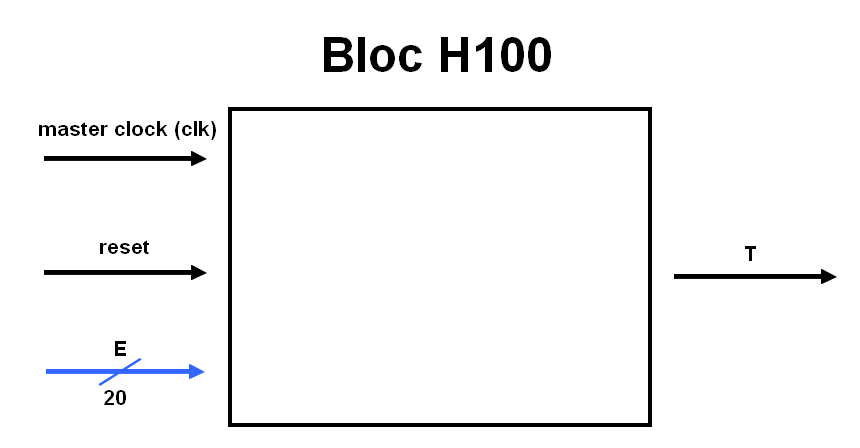
\includegraphics[width=12cm]{h100.png}
            \caption{}
        \end{figure}
    
            
        \begin{table}[h]
            \centering
            \begin{tabular}{ccccccccc}
                   \textbf{Etat} & \textbf{numéro de lignes} & sortie T \\
                     LOAD        &         5 à 6             &    0     \\
                     DECR        &         7 à 10            &    0     \\
                     TICK        &          11               &    1     \\
                \end{tabular}
        \end{table}
        
        \begin{figure}[h!]
            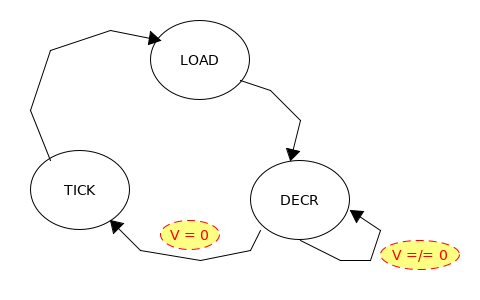
\includegraphics[width=8cm]{h100diag.png}
            \caption{}
        \end{figure}
        
        
        \newpage
        \begin{algorithm}
            \caption{Algorithme qui tourne en boucle sur le bloc}
            \begin{algorithmic}[1]
                \State \textbf{Entrée} $E$ entier sur 20 bits
                \State \textbf{Sortie} $T$ un tick codé sur 1 bit ('0' ou '1')
                \State \textbf{Registre} $R_c$ compteur sur 23 bits
                \Function{update}{}
                    \State $T = 0$
                    \State $R_c$ := $E$
                    \State \textbf{Tant que} $R_c \neq 0$
                        \State \qquad $R_c$ := $R_c - 1$
                        \State \qquad Attendre 1 master clock
                    \State \textbf{Fin tant que}
                    \State $T = 1$
                    \State Attendre 1 master clock
                \EndFunction
            \end{algorithmic}
        \end{algorithm}
        
        
        Implémentation VHDL
        \begin{lstlisting}[style=vhdl]

-------------------------------------------------------------------------------
-- Entrée:
--		clk, reset la clock et le reset
--		Entier E codé sur 21 bits (nombre de kilo master cycle)
--
--	Sortie:
--		T , le tick : '1' tous les 'E' master cycle, sinon '0'
-------------------------------------------------------------------------------

library IEEE;
use IEEE.std_logic_1164.all;
use ieee.numeric_std.all;

entity h100 is
	port(
		    clk : in STD_LOGIC;
		    reset : in STD_LOGIC;
		    E   : in  STD_LOGIC_VECTOR(20 downto 0);
		    T   : out STD_LOGIC
	    );
end h100;

architecture montage of h100 is

    -------------------------------------------------------------------------------
    --  Partie Opérative
    -------------------------------------------------------------------------------
	type T_CMD is (LOAD, DECR, NOOP);
    -- la commande courante
	signal CMD :  T_CMD; 
    -- le registre de stockage, compteur des clocks
	signal R   :  unsigned (23 downto 0);
	 -- boolean vrai si R est à 0
	signal R_IS_NULL:  STD_LOGIC;

    -------------------------------------------------------------------------------
    -- Partie Contrôle
    -------------------------------------------------------------------------------
	type STATE_TYPE is (
	ST_LOAD, ST_DECR, ST_TICK
);
signal state : STATE_TYPE;

begin

    -------------------------------------------------------------------------------
    --  Partie Opérative
    -------------------------------------------------------------------------------

	process (clk)
	begin if clk'event and clk = '1' then
		IF CMD = LOAD THEN 
			-- charges 'E' dans 'R' en kilo master cycle
			R(23 downto 3) <= unsigned(E);
			R(2  downto 0) <= to_unsigned(0, 3);
		ELSIF CMD = DECR THEN
			R <= R - 1;
		END IF;
	end if; end process;

	R_IS_NULL <= '1' WHEN R = 0 ELSE '0' ;

    -------------------------------------------------------------------------------
    -- Partie Contrôle
    -------------------------------------------------------------------------------
    -- Inputs:  R_IS_NULL, state
    -- Outputs: T, CMD, state
    -------------------------------------------------------------------------------

    -- fonction de transitition    
	process (reset, clk)
	begin
		if reset = '1' then
			state <= ST_LOAD;
		elsif clk'event and clk = '1' then
			case state is
				when ST_LOAD =>
					state <= ST_DECR ;
				when ST_DECR =>
					IF R_IS_NULL = '1' THEN
						state <= ST_TICK;
					END IF ;
				when ST_TICK =>
					state <= ST_LOAD ;
			end case;
		end if;
	end process;

    -- fonction de sortie    
	with state  select T <=
	'1'    when   ST_TICK,
	'0'    when   others;

	with state  select CMD <=
	LOAD   when   ST_LOAD,
	DECR   when   ST_DECR,
	NOOP   when   ST_TICK;

end montage;


\end{lstlisting}

\end{document}
